% \iffalse meta-comment
%
% how-to-prepare-manuscripts.txt -- CODEE Journal class example article.
%
% Copyright (C) 2009-2016  Consortium for Ordinary Differential Equations Educators.
%
% This work may be distributed and/or modified under the conditions of
% the LaTeX Project Public License, either version 1.3 of this license
% or (at your option) any later version.
%
% The latest version of this license is in
%   http://www.latex-project.org/lppl.txt
% and version 1.3 or later is part of all distributions of LaTeX
% version 2005/12/01 or later.
%
% This work has the LPPL maintenance status `maintained'.
%
% The Current Maintainer of this work is CODEE <codee@hmc.edu>
%
% This work consists of all files listed in manifest.txt.
%
% Source code available from https://github.com/hmcmathematics/codee-class/
%
% \fi
%%

%%%%%%%%%%%%%%%%%%%%%%%%%%%%%%%%%%%%%%%%%%%%%%%%%%%%%%%%%%%%%%%%%%%%%%%%%%%%%%%%%%%
% This document is a model for how to typeset documents using LaTeX               %
% for the CODEE Journal.                                                          %
%                                                                                 %
% To compile this file using LaTeX, you will need "codee.cls", which is available %
% from http://www.codee.org                                                       %
%                                                                                 %
% Compile this document using the commands                                        %
%                                                                                 %
%     pdflatex how-to-prepare-manuscripts                                         %
%     bibtex how-to-prepare-manuscripts                                           %
%     pdflatex how-to-prepare-manuscripts                                         %
%     pdflatex how-to-prepare-manuscripts                                         %
%                                                                                 %
%%%%%%%%%%%%%%%%%%%%%%%%%%%%%%%%%%%%%%%%%%%%%%%%%%%%%%%%%%%%%%%%%%%%%%%%%%%%%%%%%%%


% LaTeX Preamble (best not to change this unless you need special packages)
\documentclass{codee}
\usepackage{graphicx}
\usepackage[numbers]{natbib}
\usepackage{hyperref}
\newtheorem{theorem}{Theorem}[section]
\newtheorem{lemma}[theorem]{Lemma}
\theoremstyle{definition}
\newtheorem{definition}[theorem]{Definition}
\newtheorem{example}[theorem]{Example}
\newtheorem{problem}[theorem]{Problem}
\newtheorem{xca}[theorem]{Exercise}
\theoremstyle{remark}
\newtheorem{remark}[theorem]{Remark}
\numberwithin{equation}{section}

% Metadata for your manuscript
\title{How to Prepare Manuscripts for the CODEE Journal Using \LaTeX}
\shorttitle{Model Document}
\author{Person One and Person Two}
\affiliation{Institution A}
\author{Person Three}
\affiliation{Institution B}
\shortauthor{One, Two and Three}
\date{January 21, 2010}
\dedicatory{}
\keywords{CODEE Journal, \LaTeX}
% Put any words with special hyphenation here.
\hyphenation{Ar-thur}

% The following will be filled in by editorial staff when the paper is published on the site. 
% You do not have to fill this out now.
\submissiondate{January 21, 2010}
\publicationdate{January 21, 2010} 
\articlenumber{PA10-0000}

\begin{document}
\maketitle

% Please type in a short abstract here. Please try to avoid using any mathematical symbols
% as the abstract will also go on the CODEE Digital Library.
\begin{abstract}
  This document describes how to prepare manuscripts for the
  \emph{CODEE Journal} using \LaTeX.
\end{abstract}

% Your paper really starts here. Use \section and \subsection to
% create section headings.

\section{Introduction}

The Community of Ordinary Differential Equations Educators (CODEE)
exists to improve the teaching and learning of ordinary differential
equations (ODEs), primarily by encouraging broader use of modeling projects
and computer experiments. CODEE publishes an electronic journal
containing learning materials relating to ODEs called the
\emph{CODEE Journal}. This journal is published online at the CODEE
Digital Library, which is accessible at \url{http://www.codee.org}.


This document models how one might use the \LaTeX\ document processing
system to typeset manuscripts for publication in the \emph{CODEE
  Journal}. It is recommended that authors download the source files
for this document (including the CODEE Journal style file) and refer
to the file \texttt{how-to-prepare-manuscripts.tex} while reading this
document.

There are many wonderful print and online sources for information on the \LaTeX\ document system. Two helpful books are the classic reference by \citet{lamport-1994} and the more recent book by \citet{gratzer-2004}.

\section{Typesetting Mathematics}


\subsection{Examples of Displayed Equations}

If a ball is thrown upward from ground level with initial
velocity $v_0$, then the position $y$ of
the ball above the ground at time $t$ is given by the initial value problem
\begin{equation}\label{eq:projectile}
my'' = -mg - cy',\quad y(0)=0,\quad y'(0)=v_0,
\end{equation} 
where $m$ is the mass of the ball, $g$ is the gravitational constant,
and $c$ is the positive drag constant. Here is an example of how to
refer to equation~\eqref{eq:projectile} using the
\texttt{\textbackslash eqref} command.

Here is an example of a longer equation that must be wrapped across
several lines.

\begin{align*}
  \cos x+i\sin x &=
  \left(1-\frac{x^2}{2!}+\frac{x^4}{4!}-\frac{x^6}{6!}+\cdots+\frac{(-1)^nx^{2n}}{(2n)!}+\cdots\right) \\
&\quad+i\left(x-\frac{x^3}{3!}+\frac{x^5}{5!}-\frac{x^7}{7!}+\cdots+\frac{(-1)^{n+1}x^{2n+1}}{(2n+1)!}+\cdots\right) \\
&=1+\frac{ix}{1!}+\frac{(ix)^2}{2!}+\frac{(ix)^3}{3!}+\cdots+\frac{(ix)^n}{n!}+\cdots=e^{ix}
\end{align*}

\subsection{Systems of Differential Equations}

As you will be writing about differential equations, you will probably
find it necessary to typeset systems of differential equations. To do
so, please use the \texttt{align} environment.

Here is an example.
\begin{align}
    x' &= -ax + bxy - Hx\\
    y' &= cy - dxy - Hy
\end{align}

Here is the same example without equation numbers using the \texttt{align*} environment.
\begin{align*}
    x' &= -ax + bxy - Hx\\
    y' &= cy - dxy - Hy
\end{align*}

If you only want some of the equations to be numbered, use the \texttt{\textbackslash
  notag} command.
\begin{align}
    x' &= -ax + bxy - Hx \notag\\
    y' &= cy - dxy - Hy \label{eq:predprey-y}
\end{align}
Now we can just refer to differential equation for $y$ as
equation~(\ref{eq:predprey-y}).

If you wish to number a whole set of equations with one equation
number, use the \texttt{subequations} environment.
\begin{subequations}
\begin{align}
  \frac{dw}{dt} &= -aw \\
  \frac{dx}{dt} &= aw - bx - cxy^2 \\
  \frac{dy}{dt} &= bw - ky + cxy^2 \\
  \frac{dz}{dt} &= ky
\end{align} \label{eq:chemicalsystem}
\end{subequations}
Now we can refer to a specific equation~(\ref{eq:chemicalsystem}a) or the
whole system~\eqref{eq:chemicalsystem}.

One can include initial conditions to the right of the differential
equations by adding more alignment markers (\texttt{\&}).
\begin{align}
    x' &= -x + xy/10 - Hx, &x(0)&=8\\
    y' &= y - xy/5 -Hy,&y(0)&=16
\end{align}

\subsection{Examples and Problems}

If you would like to include sample problems or examples, you can use
the \texttt{problems} or \texttt{example} environments to easily set
these apart from the rest of your exposition.

\begin{example}
  If $a$ is a constant, the general solution to the linear
  differential equation $y'(t)=a y(t)$ is $y(t)=Ce^{at}$.
\end{example}

\begin{problem}[A sample tedious problem]\label{pr:tedious-problem}
Find the general solution to the forced differential equation $y''(x)+y(x) =
(x+1)^{20}\sin x$. You must use the undetermined coefficients
method and you are not allowed to use any technology to help
you find the answer.
\end{problem}

Notice that the numbering of these problems and examples is
automatic. Referring to them by this automatically-generated number is
easy---for example, look at Problem~\ref{pr:tedious-problem}.


\subsection{Figures}

The use of color graphics, images and other visual elements is
strongly recommended. However, color graphics should be designed with
appropriate contrast so that they can be rendered well on black and
white printers. Vector art formats such as encapsulated PostScript
(EPS) or Adobe Illustrator (AI) are preferred to raster art formats
such as JPEG, GIF or TIFF. For more information, please see
\url{http://en.wikipedia.org/wiki/Vector_art}. Figure~\ref{fig:vector-vs-raster}
gives an extreme example of the difference between vector art and
raster art.

\begin{figure}[b!] % the b! forces the figure to appear at the bottom of the page
  \centering
  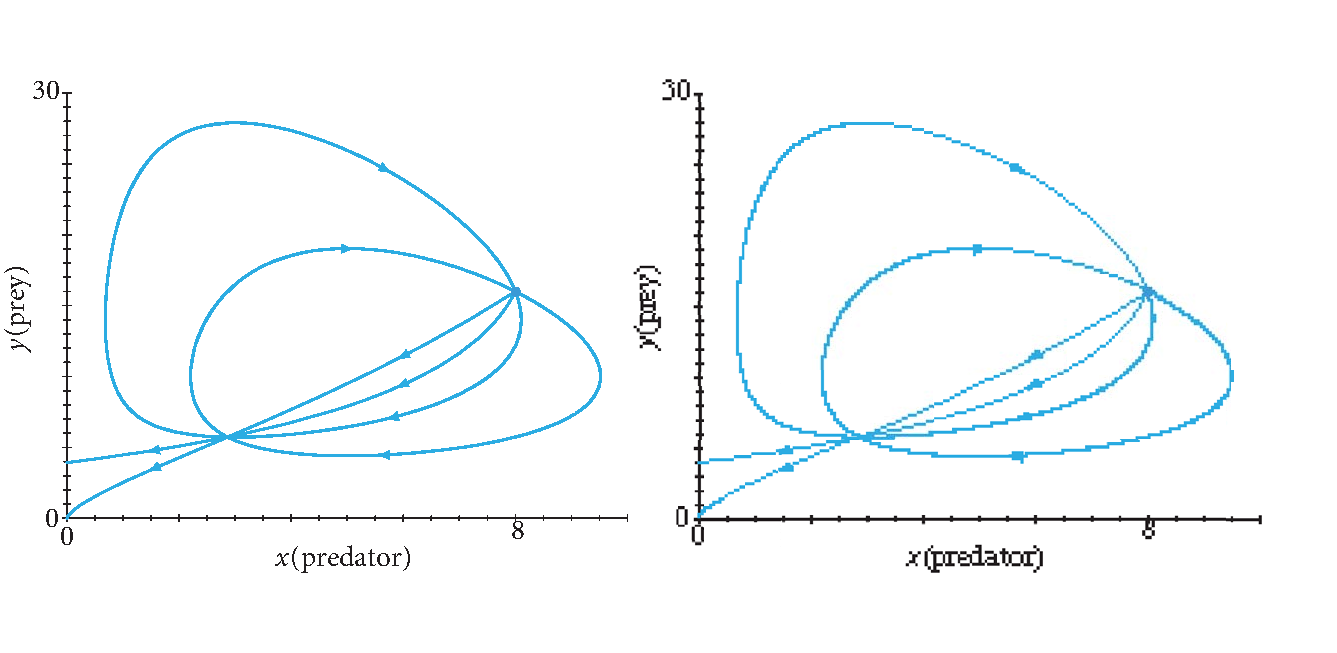
\includegraphics[width=6in,keepaspectratio=true]{vector-vs-raster}
  \caption{The figure on the right is a rasterized version of the
    figure on the left. Raster art files tend to appear pixelated and
    unattractive when the document is printed.}
  \label{fig:vector-vs-raster}
\end{figure}

If you use \texttt{pdflatex} to compile your document, your art will
need to be converted to PDF format. All graphics files should be uploaded together with
the manuscript during the submission process. 

\section{Citation Style}

The \emph{CODEE Journal} \LaTeX\ style file uses the \texttt{natbib}
package, which extends \LaTeX's own reference citation
commands. Authors should use a \texttt{.bib} file instead of the
\texttt{\textbackslash bibentry} command. Please refer to the file
\texttt{how-to-prepare-manuscripts.bib} that accompanies this
document.

Authors should use the \texttt{\textbackslash citep} and \texttt{\textbackslash citet} commands to produce parenthetical and textual citations, respectively. Here are some examples.

\begin{itemize}
\item The first paper published in the \emph{CODEE Journal} was \citet{borrelli-coleman-2009}.
\item There exist good books on the \LaTeX\ document processing system \citep{gratzer-2004,lamport-1994}.
\item Numerical methods can sometimes produce incorrect solutions to ODEs \citep{borrelli-coleman-2009}.
\item One can launch ODE Toolkit directly while viewing a PDF file \citep[see][page 5]{borrelli-coleman-2009}.
\end{itemize}

\section{Hyperlinks}

All content published by the \emph{CODEE Journal} is designed to be
as user-friendly as possible. Many users will interact with your
manuscript directly through a PDF file viewer, so it is helpful if you
can include links that will take users to helpful websites or even to
launch a piece of software.

Use the \texttt{\textbackslash url} command to add links to web
pages. If you have a system of differential equations that you would
like readers to explore using a numerical solver, consider using the
free, cross-platform numerical solver program ODE
Toolkit\footnote{\url{http://www.codee.org/software/ode-toolkit}} to
create a \texttt{.ode} file, which will allow users to interact with
your differential equations without having to retype them into the
computer. It is even possible to launch ODE Toolkit as a Java
application with your \texttt{.ode} file loaded while viewing the PDF
file.  For an example of this please see page 5 of
\url{http://www.codee.org/ref/PA09-0157/numerical-pitfalls.pdf}. These
kinds of links make it easier for instructors and students to access
software and web pages.

Notice that the \emph{CODEE Journal} style file uses the
\texttt{hyperref} package to create links that help the reader more
easily navigate through the PDF file using a PDF file viewer.  For
example, try clicking on the equation number in
``equation~\eqref{eq:projectile}'' in your PDF viewer. You should be
taken back to the page containing that equation. The \texttt{hyperref}
package also creates bookmarks from your \texttt{\textbackslash
  section} and \texttt{\textbackslash subsection} commands so that
users can quickly jump to the appropriate parts of your manuscript.

\section{Final Notes}

If you have any questions about the preparation of your manuscript,
please refer to CODEE's editorial
policy\footnote{\url{http://www.codee.org/library/editorial-policy}}
or contact the editorial staff at
\href{mailto:codee@hmc.edu}{\texttt{codee@hmc.edu}}. The editorial
policy describes the various kinds of manuscripts that are accepted by
the \emph{CODEE Journal}, the criteria will be used to review your
manuscript, and the submission process.

Before you submit your manuscript, please review this list of questions.
\begin{enumerate}
\item Does the manuscript include all of the required elements as
  described in the editorial policy? Does it address all listed criteria for peer evaluation?
\item Is all bibliographic information complete and accurate?
\item Was a spell-checking program used to catch typographic errors?
\item Have all granting or support sources been properly acknowledged?
\item Is all text in any figures, plots or diagrams readable?
\end{enumerate}

Thank you for submitting your work to the \emph{CODEE Journal}. Your
submission to the \emph{CODEE Journal} adds to the growing body of
materials on the teaching and learning of ordinary differential
equations.

% Bibliography
% This is the default CODEE Journal citation style. Please do not
% change this line.
\bibliographystyle{plainnat}
% If your bibliography file is called manuscript.bib, you would change
% "how-to-prepare-manuscripts" in the line below to "manuscript".
\bibliography{how-to-prepare-manuscripts}{}
% If you want all the items in your .bib file to be included in the
% bibliography even if they were not cited in your .tex file, then
% uncomment this line below.
\nocite{*}

\end{document}
